% 8. előadás második fele

\chapter{Az Intel Netburst architektúra}

\section{Bevezetés}
A második generációs szuperskalárok fejlesztése során a 90-es évek második felében elérték az architektúra teljesítménybeli korlátait.
A hatékonyság növelésének extenzív forrásai kimerültek.
A sebesség további fokozásához a következő módszerekkel keresték a megoldást:
\begin{itemize}
    \item új architektúrák, pl. VLIW (ld. \ref{vliw}. fejezet)
    \item párhuzamosság egyéb forrásai (szál vagy folyamat szintű párhuzamosság)
    \item frekvencia erőteljes növelése
\end{itemize}
Az Intelnél a frekvencia erőteljes növelésével próbálkoztak, de az akkori legfejlettebb architektúrájuk, a P6 (Pentium III alapja) nem volt alkalmas 1333 MHz fölötti működésre.
A fejlesztés során a 10 GHz elérését tűzték ki célul, így új architektúra kellett.
Ez lett a Netburst architektúra, amire a Pentium IV processzorcsalád épült.
Az architektúra nem jelentette a második, illetve harmadik generációs szuperskalárok gyökeres újratervezését, a célkitűzés mindössze a magasabb frekvenciás működés volt.

\section{A frekvencia növelése}
A frekvencia növeléséhez a következő változtatásokat vezették be:
\begin{itemize}
    \item Gyártási csíkszélesség csökkentése (180 nm $\rightarrow$ 65 nm), általában egy lépésben 0.7-szeresére csökkentik (így fele akkora helyen fér el ugyanannyi tranzisztor, mint a korábbi technológiánál, tehát a tranzisztorok száma megduplázható $\rightarrow$ Moore-törvény).
    \item Futószalag fokozatok hosszának csökkentése (ennek egyik módja a fokozatok kisebb részekre bontása, viszont ekkor a fokozatok száma növekszik, nő a párhuzamosan végrehajtott utasítások száma és a függőségek száma is $\rightarrow$ csökkenhet a hatékonyság).
\end{itemize}

\section{Jellemzői}
\begin{itemize}
    \item CISC architektúra (1-17 byte hosszú utasítások)
    \item belső RISC mag
    \item hosszabb futószalagok (több függőség, de magasabb frekvencia)
\end{itemize}

\section{Újdonságok}
\begin{itemize}
    \item Execution Trace Cache: L1 utasítás cache-nek felel meg, de CISC helyett már dekódolt RISC utasításokat tartalmaz a végrehajtásuk feltételezett sorrendjében.
    \item Hyper futószalag technológia: a dekódoló fokozat nincs benne, a dekódolás futószalagon kívül történik, azért, hogy az L1 cache-ben már dekódolt és átalakított utasítások szerepelhessenek.
    \item 20-31 fokozatú futószalag (korábban 10-15 fokozat) - hátrány, hogy hibás becslés esetén nagyobb a büntetés, több fokozatot kell törölni a futószalagból $\rightarrow$ fajlagos teljesítmény csökkenés.
    \item Enhanced Branch Prediction: továbbfejlesztett elágazásbecslő logika, 94-97 \%-os hatékonyság (PIII-hoz képest kb. 33 \%-al csökkent a hibás becslések száma).
    \item Quad Data Rate Bus: belső rendszerbusz, gyorsítja az adatelérést az L1 és L2 gyorsítótárak felé. A buszfrekvencia négyszeresén továbbítja az adatokat (a külső rendszerbusz sebességét nem lehetett növelni, mivel a memória nem gyosult jelentősen). Ennek eléréséhez kettő órajel generátort alkalmaz, 90\textdegree-os fáziseltolással, valamint a felfutó és lefutó élen is történik adattovábbítás. Így óraciklusonként négy adattovábbítás történik. Ezt a működést mutatja be a \ref{fig:qdrb}. ábra.
\end{itemize}
\begin{figure}[h]
    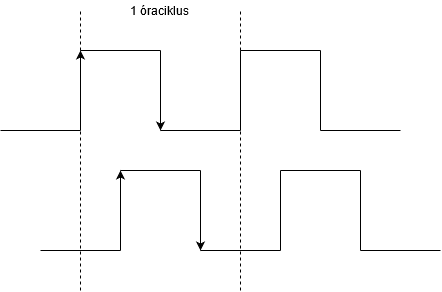
\includegraphics[width=0.6\textwidth]{qdrb}
    \centering
    \caption{A Quad Data Rate Bus kettős órajele}
    \label{fig:qdrb}
\end{figure}